\documentclass[10pt, a5paper]{article}
\usepackage{pdfpages}
\usepackage{parallel}
\usepackage[T2A]{fontenc}
\usepackage{ucs}
\usepackage[utf8x]{inputenc}
\usepackage[polish,english,russian]{babel}
\usepackage{hyperref}
\usepackage{rotating}
\usepackage[inner=2cm,top=1.8cm,outer=2cm,bottom=2.3cm,nohead]{geometry}
\usepackage{listings}
\usepackage{graphicx}
\usepackage{wrapfig}
\usepackage{longtable}
\usepackage{indentfirst}
\usepackage{array}
\newcolumntype{P}[1]{>{\raggedright\arraybackslash}p{#1}}
\frenchspacing
\usepackage{fixltx2e} %text sub- and superscripts
\usepackage{icomma} % коскі ў матэматычным рэжыме
\PreloadUnicodePage{4}

\newcommand{\longpage}{\enlargethispage{\baselineskip}}
\newcommand{\shortpage}{\enlargethispage{-\baselineskip}}

\def\switchlang#1{\expandafter\csname switchlang#1\endcsname}
\def\switchlangbe{
\let\saverefname=\refname%
\def\refname{Літаратура}%
\def\figurename{Іл.}%
}
\def\switchlangen{
\let\saverefname=\refname%
\def\refname{References}%
\def\figurename{Fig.}%
}
\def\switchlangru{
\let\saverefname=\refname%
\let\savefigurename=\figurename%
\def\refname{Литература}%
\def\figurename{Рис.}%
}

\hyphenation{admi-ni-stra-tive}
\hyphenation{ex-pe-ri-ence}
\hyphenation{fle-xi-bi-li-ty}
\hyphenation{Py-thon}
\hyphenation{ma-the-ma-ti-cal}
\hyphenation{re-ported}
\hyphenation{imp-le-menta-tions}
\hyphenation{pro-vides}
\hyphenation{en-gi-neering}
\hyphenation{com-pa-ti-bi-li-ty}
\hyphenation{im-pos-sible}
\hyphenation{desk-top}
\hyphenation{elec-tro-nic}
\hyphenation{com-pa-ny}
\hyphenation{de-ve-lop-ment}
\hyphenation{de-ve-loping}
\hyphenation{de-ve-lop}
\hyphenation{da-ta-ba-se}
\hyphenation{plat-forms}
\hyphenation{or-ga-ni-za-tion}
\hyphenation{pro-gramming}
\hyphenation{in-stru-ments}
\hyphenation{Li-nux}
\hyphenation{sour-ce}
\hyphenation{en-vi-ron-ment}
\hyphenation{Te-le-pathy}
\hyphenation{Li-nux-ov-ka}
\hyphenation{Open-BSD}
\hyphenation{Free-BSD}
\hyphenation{men-ti-on-ed}
\hyphenation{app-li-ca-tion}

\def\progref!#1!{\texttt{#1}}
\renewcommand{\arraystretch}{2} %Іначай формулы ў матрыцы зліпаюцца з лініямі
\usepackage{array}

\def\interview #1 (#2), #3, #4, #5\par{

\section[#1, #3, #4]{#1 -- #3, #4}
\def\qname{LVEE}
\def\aname{#1}
\def\q ##1\par{{\noindent \bf \qname: ##1 }\par}
\def\a{{\noindent \bf \aname: } \def\qname{L}\def\aname{#2}}
}

\def\interview* #1 (#2), #3, #4, #5\par{

\section*{#1\\{\small\rm #3, #4. #5}}

\def\qname{LVEE}
\def\aname{#1}
\def\q ##1\par{{\noindent \bf \qname: ##1 }\par}
\def\a{{\noindent \bf \aname: } \def\qname{L}\def\aname{#2}}
}

\begin{document}
\title{Обзор GNURadio}
\author{Юрий Адамов, Минск, Беларусь\footnote{\url{begemotv2718@tut.by}, \url{http://lvee.org/ru/abstracts/115}}}
\maketitle
\begin{abstract}
Gnuradio is a software framework intended in particular to building software defined radio. New functions and new external devices can be added easily by writing plugins. It also has graphical front end to rapidly create software signal processors.
I will demonstrate creating software radio receivers with GNUradio and commodity components.
Also I will discuss using gnuradio as a general signal processing tool and writing plugins for gnuradio, using processing of electroencephalogram (EEG) as an example.
\end{abstract}
\subsection*{От обычного радио к программно определяемому радио}

Изначально все компоненты радиоприемников и радиопередатчиков создавались из дискретных компонент. Из отдельных катушек, резисторов,  конденсаторов, транзисторов и т.п. собирались устройства, которые применяли определенные математические преобразования к исходному сигналу, принятому в антенне, дабы получить какой-то полезный сигнал на выходе. Например, типичный супергетеродинный приемник осуществляет предварительное усиление сигнала (умножение на константу в идеале), преобразование частоты (перемножение исходного сигнала и сигнала внутреннего генератора "--- гетеродина), фильтрацию получившегося сигнала полосовым фильтром, детектирование сигнала.

Возьмем более сложную систему "--- телевизор. Он также может быть описан как совокупность сравнительно простых блоков, осуществляющих простые математические преобразования сигнала: перенос телевизионного сигнала на промежуточную частоту (гетеродин "--- смеситель), усиление полного сигнала на промежуточной частоте (фильтр, усилитель), выделение несущих звука и изображения (фильтры), детектирование звука и изображения (AM детектор, FM детектор), усилители, выделение сигналов цветности (фильтры), детектирование сигналов цветности (FM детекторы), линии задержки (фазовый преобразователь), сумматоры (восстановление R,\,G,\,B), схемы синхронизации (пороговый детектор).

Несмотря на чисто аналоговую элементную базу, проектирование сложного радиоэлектронного прибора подобно проектированию программной системы "--- мы разбиваем систему на слабосвязанные функциональные блоки, блоки разбиваем на подблоки, пока не дойдем до элементарных операций (усиления, фильтрации, детектирования, порогового детектирования и т.д.).

Сейчас, когда частоты цифровой электроники уже довольно глубоко в радиодиапазоне, стало возможным сначала преобразовать сигнал из антенны в цифровую форму и затем делать многие из перечисленных выше операций уже на цифровых процессорах. При этом проектирование системы можно устраивать как средствами обычных языков программирования, так и с помощью старых добрых блок-схем.

Программно-определяемые радиосистемы, собственно, и предназначены для такой задачи. Gnuradio "--- как раз представитель подобного класса систем.

Рассмотрим чуть подробнее возможности современного процессора по обработке радиосигнала. Если мы возьмем диапазон длинных волн (30-300 кГц, километровые волны), то за один период этого сигнала успевает пройти более 10000 тактов процессора. Этого более чем достаточно, чтобы сделать с сигналом все что угодно (например, принять одновременно все длинноволновые станции и записывать каждую из них в отдельный файл). При этом процессор справится даже если мы добавим к ДВ существенный кусок средневолнового диапазона (300 кГц -- 3 МГц). Однако выполнить то же самое с наиболее интересными коротковолновым, УКВ и СВЧ диапазонами так просто не получится: в запасе остается слишком мало тактов. Здесь приходится использовать компромисс: с помощью аналоговой электроники часть представляющего интерес диапазона можно перенести по частоте в диапазон от 0 до нескольких мегагерц, а потом уже этот сигнал оцифровывать и обрабатывать с помощью программно-определяемого радио.

Практически те же самые средства, как программные так и аппаратные, работают и в обратную сторону "--- для подготовки к передаче сигнала в эфир.

Предварительное преобразование и оцифровку сигнала делает специальная аппаратура Universal software radio peripheral (USRP, универсальное внешнее устройство для программного радио). Она содержит в себе предварительный усилитель, преобразователь частоты и АЦП. До недавнего времени это были специализированные и потому сравнительно дорогие устройства (например, USRP фирмы Ettus research стоит порядка \textbackslash{}\$700). Однако несколько лет назад были открыты свойства USRP у сравнительно дешевых устройств для приема DVB-T телевидения на базе чипов Elonics E4000 и Raphael Micro R820T. Эти устройства стоят порядка \textbackslash{}\$20, имеют довольно широкий диапазон частот настройки (54---2200 МГц у E4000, 24---1700 МГц у R820T), большую частоту выборки АЦП (2.5 Ms/s) и приемлемую чувствительность. Недостатки таких приемников DVB-T "--- закрытость и невозможность передачи сигнала. Подобных недостатков лишен проект HackRF "--- свободное аппаратное обеспечение с возможностью приема и передачи. Однако, HackRF дороже и может вызвать претензии у служб радиоконтроля и таможни (поскольку является передатчиком).

\subsection*{Архитектура Gnuradio}

Все схемы в GNUradio строятся из \emph{блоков}. Блок "--- это элементарная единица обработки сигнала, «черный ящик» с несколькими входами и выходами. Выходы одних блоков можно соединять с однотипными входами других блоков, строя блок-схемы. Блоки можно соединять как программно (внутри программ на Python или C++) так и в графическом редакторе (GNURadio companion). Алгоритм обработки сигнала внутри блока реализуется на C++ (с ассемблерными вставками), для всех блоков существует обвязка на Python.

Блоки делятся на источники (sources), потребители (sinks), промежуточные и т.д. Также имеется большая библиотека графических виджетов, оформленных в виде блоков (поддерживаются Wx- и QT-виджеты).

Источники не имеют входов, зато имеют выходы. К источникам относятся интерфейсы USRP-приемников, программные генераторы сигналов, интерфейсы к микрофонам звуковой карточки, файлы с записями сигналов\ldots{} Например, описанные в предыдущем разделе приемники DVB-T  обрабатываются блоком RTL-SDR.

Потребители (sinks) не имеют выходов, но имеют один или несколько входов. К потребителям относят интерфейсы USRP-передатчиков, выходы звуковой карточки, выводы в файл. Некоторые графические виджеты также относятся к потребителям (например анализатор спектра, осциллограф).

Имеются потребители и источники, конвертирующие сигнал в/из TCP или UDP-поток данных. С помощью таких блоков можно разделить обработку сигнала на несколько машин.

Типичный представитель промежуточных блоков "--- фильтр. Имеется полный набор стандартных FIR или IIR-фильтров. Также фильтры могут конвертировать частоту выборки сигнала (децимация). Еще один класс промежуточных блоков "--- детекторы.

Имеются также вспомогательные блоки "--- например, представляющие глобальные переменные или виджеты для настройки глобальных переменных.

Для примера разберем, как сделать работающий FM-приемник из стандартных компонент GNUradio. Блок-схема самого простого приемника показана на рисунке.  Он состоит из источника (RTL-SDR), фильтра нижних частот (селектор сигнала одной станции), FM-детектора, еще ресэмплера и потребителя "--- аудиокарточки. Частота настройки и частота выборки задаются глобальными переменными. Для удобства работы добавим виджеты настройки и красивую картинку для спектра сигнала. Чтобы превратить эту схему в приемник AM-сигнала, достаточно заменить детектор. Можно устроить одновременный прием двух FM станций, если они помещаются в полосу частот 1 MГц. Для этого можно использовать блок сдвига частоты frequency XLATE.

\begin{center}
  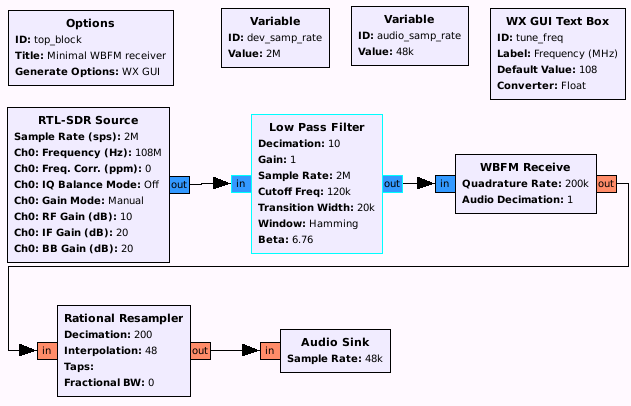
\includegraphics[width=\textwidth]{112_2014_w_Adamov_struct.png}
\end{center}

\subsection*{Нестандартные применения GNUradio и написание своих блоков}

Хотя проект GNUradio изначально предназначен для задач обработки радиосигналов, он предоставляет набор стандартных хорошо оптимизированных компонент, пригодных для любой цифровой обработки сигналов. В качестве еще одного примера рассмотрим, как можно обработать данные энцефалограммы человека (запись мозговой активности). Для анализа в энцефалограмме выделяют несколько ритмов, они лежат в разных диапазонах частот (альфа 8---13 Гц, бета 13---30 Гц, гамма \textgreater{} 30 Гц, тета и дельта 1---7 Гц). Для определения активности в этих каналах нужно отфильтровать соответствующие диапазоны частот, по возможности сдвинуть частоты к нулю, продетектировать и усреднить сигнал. Однако данные от энцефалографа поступают в виде csv-файла, который стандартные средства GNUradio читать не умеют. С помощью gr\_modtool мы создаем шаблон нового компонента

\verb!% gr_modtool newmod csvfile!

Добавляем источник с типом выходных данных float (f).

\verb!% cd gr_csvfile!

\verb!% gr_modtool add -t source csvfile_f!

Это создает структуру директорий:

\verb!% ls gr_csvfile!

\verb!apps cmake CMakeLists.txt docs examples!

\verb!grc include lib python swig!

Нам в первую очередь потребуется отредактировать файлы \textbf{сsv\-file\_f\_impl.cc} и \textbf{csvfile\_f\_impl.h}. В качестве образца возьмем стандартный компонент чтения из wav-файла, который есть в исходных кодах GNUradio. Нужно также отредактировать xml-файл описания компонента в директории grc. Далее, после компиляции с помощью cmake, получаем нужный компонент.

\end{document}
